% ====================================================================
%%- Archivo de ejemplo: Capítulo 1 -%%
% ====================================================================
% Creado por: Francisco Alberto Sandoval Noreña
% e-mail: fasandoval@utpl.edu.ec
% 
% Version 1.1.0
% Date: 07/11/2019
%
% Fecha de creación: 11 de noviembre de 2018
% Version: 0.1
% ====================================================================
%

\chapter{FORMATO DE LOS CAPÍTULOS}

\section{Descripción de la plantilla}

%La plantilla puede descargarse en la siguiente dirección web: 



\section{Cómo iniciar la escritura de una tesis nueva con la plantilla}
Los pasos que debe seguir para empezar la escritura de una tesis nueva con la plantilla \texttt{ThesisUTPL.cls} son los siguientes: 

\begin{enumerate}
	\item Descargar los documentos de la plantilla de \url{https://github.com/fasandovaln/ThesisUTPL}.
	\item Duplicar la carpeta de ejemplo que ha descargado. 
	\item Abrir el fichero ``\lstinline|main_Thesis.tex|'' con su editor preferido de \LaTeX.
	\item Guarde el archivo con un nuevo nombre. 
	\item Antes de realizar cualquier cambio, compile el archivo para verificar que no existe ningún error. Luego de la compilación debería obtener como resultado un documento similar a este. Puede requerir instalar nuevos paquetes a su distribución o actualizarla para compilar correctamente. 
	\item Seleccione las opciones de la clase de acuerdo a su necesidad. 
	\item Modifique la información básica de acuerdo a su caso. 
	\item Tenga en cuenta que se ha creado una carpeta para las figuras y otra para los documentos. Trate de mantener ese orden. En la carpeta ``DOCUMENTS'' se encuentran archivos ``\texttt{.tex}'' que corresponden a las diferentes partes del documento. 
	\item Escriba cada capítulo en un fichero ``\texttt{.tex}'' independiente y guárdelo en la carpeta ``DOCUMENTS''. Agréguelos en el punto del documento deseado utilizando para ello el comando:
	\begin{center}
		\lstinline|\input{DOCUMENTS/nombre_del_fichero.tex}|.
	\end{center}
	\item Utilice las indicaciones dadas en este capítulo para el manejo de figuras, tablas, ecuaciones, etc. Además, recuerde compilar frecuentemente el documento. 
	\item \textbf{Sugerencia:} Recuerde revisar, previo a la presentación final de su tesis en Biblioteca, el repositorio de la plantilla, ya que se realizan actualizaciones en relación a los cambios sugeridos por Biblioteca o los errores reportados. 
\end{enumerate}

\section{Estructura del documento que se genera}
El documento final generado (en formato PDF) tendrá la siguiente estructura:

\begin{itemize}
	\item \textbf{Carátula}. La información de la carátula se modifica en el archivo principal en la sección: Información básica del documento.  
	\item \textbf{Aprobación del Director del Trabajo de Titulación}. La información se genera automáticamente, no es necesario realizar cambios. 
	\item \textbf{Declaración de Autoría y Cesión de Derechos}. La información se genera automáticamente, no es necesario realizar cambios. 
	\item \textbf{Dedicatoria}. La información de la dedicatoria puede ser ingresada en el archivo PRE-CAPÍTULOS. 
	\item \textbf{Agradecimiento}. La información de los agradecimientos puede ser ingresado en el archivo PRE-CAPÍTULOS. 
	\item \textbf{Índice de Contenidos}. El Índice de Contenidos se genera automáticamente. 
	\item \textbf{Lista de Figuras}. La Lista de Figuras se genera automáticamente. 
	\item \textbf{Lista de Tablas}. La Lista de Tablas se genera automáticamente. 
	\item \textbf{Resumen y Palabras Claves}. La información del Resumen y las Palabras Claves puede ser ingresado en el archivo PRE-CAPÍTULOS.
	\item \textbf{Abstract and Keywords}. La información del Abstract y los Keywords puede ser ingresado en el archivo PRE-CAPÍTULOS.
	\item \textbf{Lista de Abreviaturas}. (Opcional) La información de la Lista de Abreviaturas puede ser ingresada en el archivo PRE-CAPÍTULOS. Si no va a utilizar esta sección puede comentarla. 
	\item \textbf{Lista de Símbolos}. (Opcional) La información de la Lista de Símbolos puede ser ingresada en el archivo PRE-CAPÍTULOS. Si no va a utilizar esta sección puede comentarla. 
	\item \textbf{Introducción}. Emplee el archivo INTRODUCCIÓN que se encuentra en la carpeta DOCUMENTS para escribir la introducción. Puede emplear secciones, subsecciones o párrafos, sin embargo, estos no se numeran. 
	\item \textbf{Capítulos de la Tesis}. Se recomienda escribir cada capítulo en un archivo diferente. Los capítulos agregados aquí son únicamente de ejemplo. Usted puede comentarlos y agregar sus archivos.  
	\item \textbf{Conclusiones}. Las conclusiones deben ser agregadas en el archivo CONCLUSIONES que se encuentra en la carpeta DOCUMENTS. Igual que la Introducción puede emplear secciones o subsecciones pero estas no se numerarán.  
	\item \textbf{Recomendaciones}. Las recomendaciones deben ser agregadas en el archivo RECOMENDACIONES que se encuentra en la carpeta DOCUMENTS. Igual que la Introducción puede emplear secciones o subsecciones pero estas no se numerarán.   	
	\item \textbf{Bibliografía}. Se puede escoger entre dos estilos para citar: APA o IEEE.
	\item \textbf{Anexos}. Se recomienda crear los Anexos en archivos separados. El archivo ANEXO1 es un ejemplo que puede comentar para incluir su información.   
\end{itemize}

\section{Clase de documento y opciones}

Para utilizar la plantilla se debe emplear la clase creada para el efecto de la siguiente manera: 

\lstinline|\documentclass[unAutor, APA, hiperenlaces]{ThesisUTPL}| 

Las posibles opciones con las que se puede configurar el documento son: 

\begin{enumerate}
	\item \textbf{Cantidad de autores de la tesis:} Se emplea para indicar la cantidad de autores de la tesis. Esto genera algunos cambios en la carátula, y páginas iniciales que son generadas automáticamente. \\
	\textit{Opciones posibles:} ``unAutor'', ``dosAutores'', ``tresAutores''. \\
	\textit{Valor por defecto:} ``unAutor''.
	%
	\item \textbf{Estilo de Bibliografía:} Permite determinar el estilo para la bibliografía y las citas en el texto. \\
	\textit{Opciones posibles:} ``APA'', ``IEEE''.\\
	\textit{Valor por defecto:} ``APA''. \\
	\textit{Nota:} Por favor considerar las instrucciones de compilación sugeridas en la Sección \ref{sec:Bibliografia}.
	
	\item \textbf{Hiperenlaces:} Permite habilitar los hiperenlaces a lo largo de todo el documento. Esto cubre el índice de contenidos, enlaces url, citas, y otros. \\
	\textit{Opción posible:} ``hiperenlaces''. 
	
\end{enumerate}

\section{Paquetes empleados en la plantilla}

A continuación se presenta los paquetes empleados en la plantilla. Usted puede agregar paquetes adicionales de acuerdo a su necesidad en el archivo ``\lstinline|0_PREAMBULO.tex|'' que se encuentra en la carpeta ``DOCUMENTS''. Sin embargo, recuerde que algunos paquetes pueden ser incompatibles con otros por lo que es importante que verifique si el paquete que va a agregar es compatible con los empleados en la plantilla. Los paquetes empleados son los siguientes: 

\begin{longtable}{p{.18\textwidth} p{0.82\textwidth}}
	\texttt{ifthen}  	& \textit{Conditional commands in LaTeX documents.}  \\  
	\texttt{inputec} 	& \textit{Accept different input encodings. Opción: utf8.} \\ 
	\texttt{fontenc} 	& \textit{Standard package for selecting font encodings. Opción: T1.} \\
	\texttt{setspace}   & \textit{Spacing between lines} \\ 
	\texttt{babel} 	 	& \textit{Simplified Spanish support for Babel (hyphenation). Opción: spanish.} \\
	\texttt{helvet}  	& \textit{URW Arial font pack for use with LATEX. Opción: scaled}\\
	\texttt{amsmath} 	& \textit{Soport math simbols-fonts.} \\
	\texttt{amssymb}    & \textit{Soport math simbols-fonts.}\\
	\texttt{amsfonts} 	& \textit{Soport math simbols-fonts.}\\
	\texttt{latexsym} 	& \textit{Soport math simbols-fonts.}\\
	\texttt{graphicx} 	& \textit{Enhanced support for graphics.}\\
	\texttt{xcolor} 	& \textit{Driver-independent color extensions for LATEX and pdfLATEX. Opciones: x11names, table.} \\
	\texttt{subfigure} 	& \textit{Figures divided into subfigures.} \\
	\texttt{longtable} 	& \textit{Allow tables to flow over page boundaries.} \\
	\texttt{multirow}  	& \textit{Create tabular cells spanning multiple rows.} \\
	\texttt{booktabs} 	& \textit{Publication quality tables in LATEX} \\
	\texttt{listings} 	& \textit{source code printer for LATEX }	 \\
	\texttt{enumitem} 	& \textit{Customize lists} \\
	\texttt{morefloats} & \textit{Increase the number of simultaneous LATEX floats. Opción: maxfloats=25.} \\
	\texttt{url} 		& \textit{Verbatim with URL-sensitive line breaks. Opción: hyphens.} \\
	\texttt{hyperref} 	& \textit{Extensive support for hypertext in LATEX. Opción: breaklinks=true.} \\
	\texttt{titlesec} 	& \textit{Modify title format.} \\
	\texttt{appendix}   & \textit{Modifying the typesetting of appendix titles.} \\
	\texttt{vmargin} 	& \textit{Margins and paper sizes.} \\
	\texttt{fancyhdr} 	& \textit{Page layout.}\\
	\texttt{caption} 	& \textit{The caption package provides many ways to customise the captions infloating environments such figure and table.}\\
	\texttt{natbib} 	& \textit{package that implements both author-year and numbered references.}

\end{longtable} 


\section{Particularidades de la plantilla}

A continuación se presenta algunos ejemplos de opciones que pueden usarse en el transcurso de la redacción, a saber: figuras, tablas, referencias, ecuaciones, etc. 

\subsection{Figuras}

Para las figuras emplee el entorno ``figure'' según el ejemplo mostrado en la Fig. \ref{fig:utplcruz}. Emplee el comando \lstinline|\captionsetup{width=n\textwidth}| donde ``n'' es un número entre 0 y 1 que representa el espacio que ocupa el título de la figura en relación al ancho del texto. Este parámetro debe ajustarse en razón del tamaño de la figura respecto al ancho de la página. Por otra parte, el comando \lstinline|\FigExtraCaptionUTPL{}{}| permite introducir la ``Fuente'' y ``Elaborado por'', respectivamente. Los demás comandos son los habituales. 

Para referirse a una figura en el texto emplee el comando \lstinline|\ref{}| incluyendo la etiqueta que corresponda. También se puede emplear el comando \lstinline|\autoref{}|, por ejemplo: \autoref{fig:utplcruz}. La diferencia radica en que al emplear  \autoref{fig:utplcruz} el comando agrega la palabra reservada según el tipo de entorno que se utilice, en este caso, ``Figura''. Cuando emplea \lstinline|\ref{}| usted debe agregar la palabra ``Figura'' por teclado. 

\begin{figure}[h!]
	\centering
	\captionsetup{width=0.7\textwidth}
	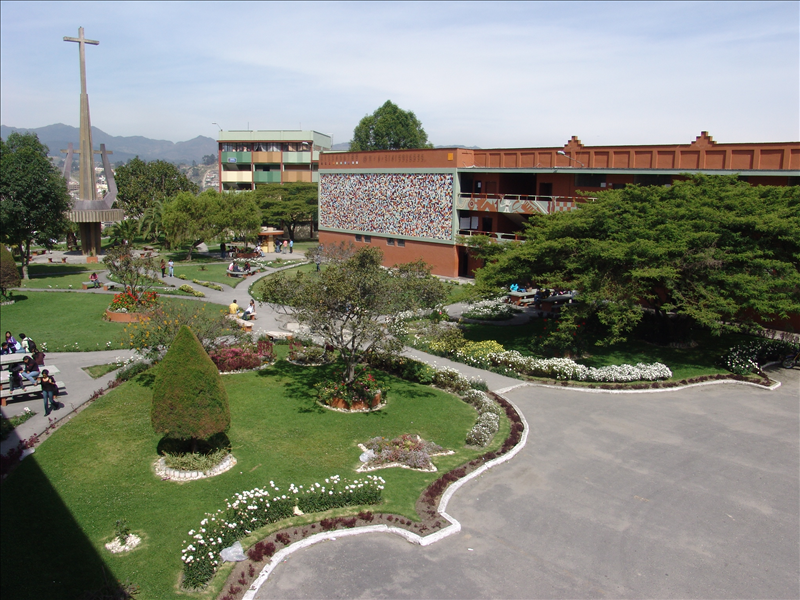
\includegraphics[width=0.7\linewidth]{FIGURES/UTPL_cruz}
	\caption{Campus UTPL}
	\FigExtraCaptionUTPL 			% \FigExtraCaptionUTPL{''Fuente''}{''Elaboración''}
		{\cite{utpl2008campus}}		% Fuente
		{UTPL}			% Elaboración
	\label{fig:utplcruz}
\end{figure}

\begin{figure}[h!]
	\centering
	\captionsetup{width=0.9\textwidth}
	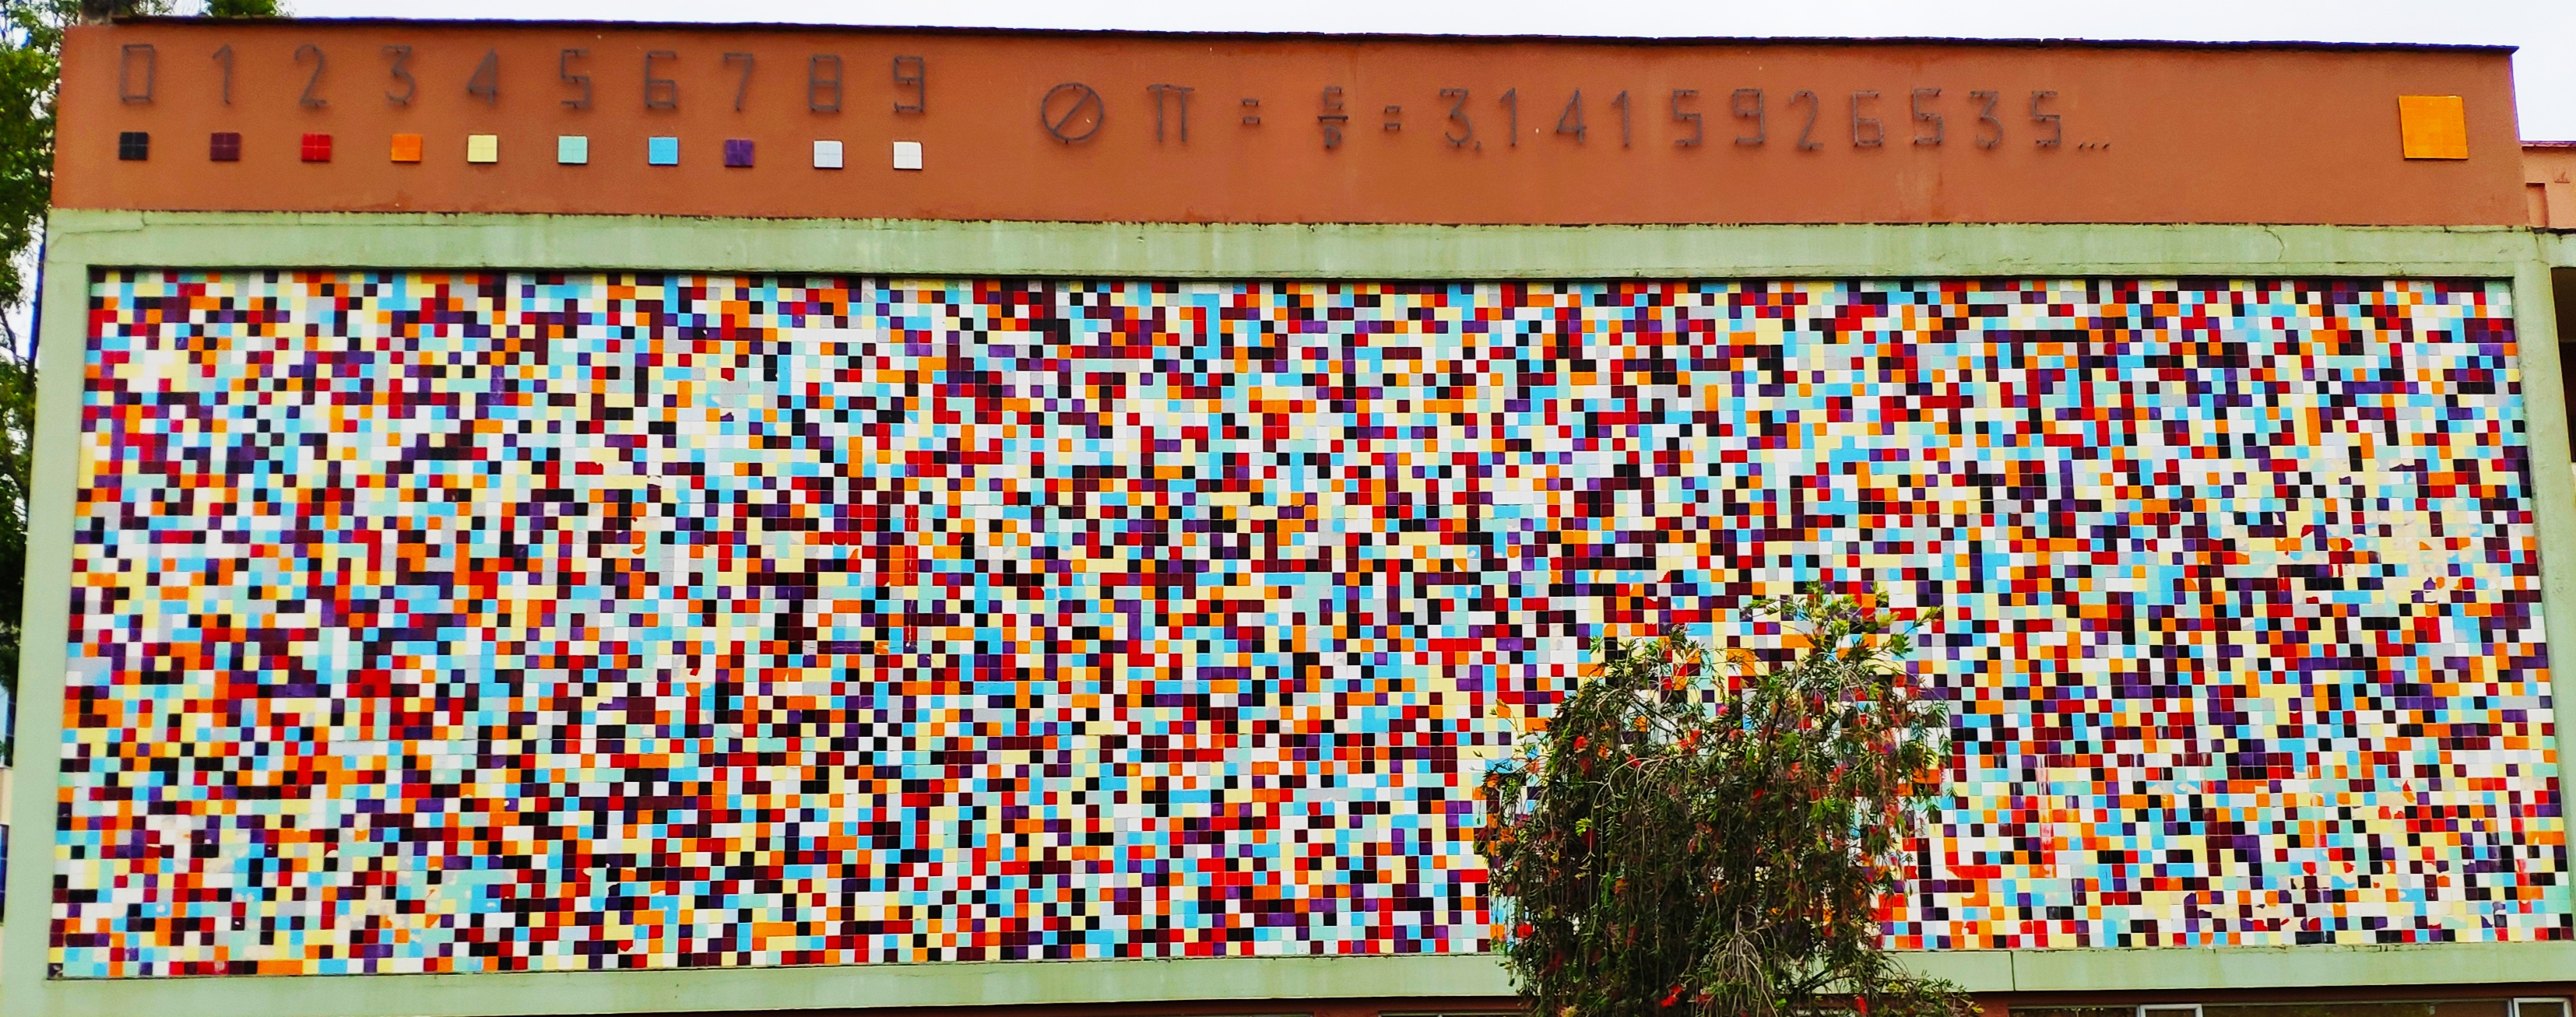
\includegraphics[width=0.9\linewidth]{FIGURES/UTPL_MuralPi}
	\caption{Mural del número $ \pi $ en el Campus de la UTPL: Mosaico de 1800 cifras decimales diseñado por Hno. Ticiano García (1974).}
	\FigExtraCaptionUTPL 			% \FigExtraCaptionUTPL{''Fuente''}{''Elaboración''}
	{Autor}		% Fuente
	{Autor}      % Elaboración
	\label{fig:utplcruz2}
\end{figure}

Además, recuerde que está incluido en la plantilla el paquete \texttt{subfigure} que le permite incluir sub-figuras en el texto. 

\subsection{Tablas}
Para la elaboración de tablas se recomienda usar el entorno ``table''. De acuerdo al ejemplo presentado (ver Tabla \ref{tb:Ejemplo}). Emplee el comando \lstinline|\captionsetup{width=n\textwidth}| donde ``n'' es un número entre 0 y 1 que representa el espacio que ocupa el título de la tabla en relación al ancho del texto. Este parámetro debe ajustarse en razón del tamaño de la tabla respecto al ancho de la página. Por otra parte, el comando \lstinline|\FigExtraCaptionUTPL{}{}| permite introducir la ``Fuente'' y ``Elaboración'', respectivamente. Los demás comandos son los habituales. 

Para referirse a una tabla en el texto emplee el comando \lstinline|\ref{}| incluyendo la etiqueta que corresponda. También se puede emplear el comando \lstinline|\autoref{}|, por ejemplo: \autoref{tb:Ejemplo}.

\begin{table}[]
	\centering
	\captionsetup{width=0.44\textwidth}
	\caption{Ejemplo de tabla}
	\label{tb:Ejemplo}
	\begin{tabular}{|l|l|l|}
		\hline
		\textbf{Columna 1} & \textbf{Columna 2} & \textbf{Columna 3} \\ \hline
		ítem 1             & ítem 2             & ítem 3             \\ \hline
		ítem 4             & ítem 5             & ítem 6             \\ \hline
		ítem 7             & ítem 8             & ítem 9             \\ \hline
	\end{tabular}
	\vspace{3pt}
	\FigExtraCaptionUTPL		% \FigExtraCaptionUTPL{''Fuente''}{''Elaboración''}	
		{Autor}					% Fuente
		{Autor} 				% Elaboración			
\end{table}

En el caso de tener en su texto tablas extensas de más de una página, puede emplear el entorno \lstinline|longtable| cuyo paquete ya se encuentra adicionado al formato. Sin embargo, debe emplear \lstinline|\FigExtraCaptionUTPLLongtable{}{}| para agregar la fuente y la elaboración. En la \autoref{tb:TablaLarga} se presenta un ejemplo. 

\begin{longtable}{|c|c|c|c|}
	\captionsetup{width=0.9\textwidth}
	\caption{Un ejemplo simple de tabla larga} 	
	\label{tb:TablaLarga}\\
	\hline
	\textbf{Primera columna} & \textbf{Segunda columna} & \textbf{Tercera columna} & \textbf{Cuarta columna} \\
	\hline
	\endfirsthead
%	\multicolumn{4}{c}%
	\caption*{\tablename{} \thetable: (continuación)} \\

	\hline
	\textbf{Primera columna} & \textbf{Segunda columna} & \textbf{Tercera columna} & \textbf{Cuarta columna} \\
	\hline
	\endhead
%		\hline
	\endlastfoot
	1 & 2 & 3 & 4 \\ 1 & 2 & 3 & 4 \\ 1 & 2 & 3 & 4 \\ 1 & 2 & 3 & 4 \\
	1 & 2 & 3 & 4 \\ 1 & 2 & 3 & 4 \\ 1 & 2 & 3 & 4 \\ 1 & 2 & 3 & 4 \\
	1 & 2 & 3 & 4 \\ 1 & 2 & 3 & 4 \\ 1 & 2 & 3 & 4 \\ 1 & 2 & 3 & 4 \\
	1 & 2 & 3 & 4 \\ 1 & 2 & 3 & 4 \\ 1 & 2 & 3 & 4 \\ 1 & 2 & 3 & 4 \\
	1 & 2 & 3 & 4 \\ 1 & 2 & 3 & 4 \\ 1 & 2 & 3 & 4 \\ 1 & 2 & 3 & 4 \\
	1 & 2 & 3 & 4 \\ 1 & 2 & 3 & 4 \\ 1 & 2 & 3 & 4 \\ 1 & 2 & 3 & 4 \\
	1 & 2 & 3 & 4 \\ 1 & 2 & 3 & 4 \\ 1 & 2 & 3 & 4 \\ 1 & 2 & 3 & 4 \\
	1 & 2 & 3 & 4 \\ 1 & 2 & 3 & 4 \\ 1 & 2 & 3 & 4 \\ 1 & 2 & 3 & 4 \\
	\hline
	\FigExtraCaptionUTPLLongtable % \FigExtraCaptionUTPL{''Fuente''}{''Elaboración''}	
		{Autor}					% Fuente
		{Autor} 				% Elaboración	
\end{longtable}


\subsection{Ecuaciones}
Para las ecuaciones numeradas emplee el entorno ``equation'' (ver \eqref{eq:Ecuacion_Shannon-Hartley}). Las ecuaciones se numeran por capítulo. Emplee  \lstinline|\eqref{}| para referirse a una ecuación particular.  

\begin{equation}\label{eq:Ecuacion_Shannon-Hartley}
C = B \log_{2} \left( 1 + \frac{S}{N} \right) 
\end{equation}


\subsection{Bibliografía}
\label{sec:Bibliografia}
La plantilla permite utilizar dos estilos para citar, a saber: APA e IEEE. Pueden elegirse como opción de la clase \textit{ThesisUTPL}. El estilo APA se encuentra por defecto. Para citar empleando el estilo APA se utiliza \textit{natbib} y para el estilo IEEE \textit{bibtex}. 

Puede agregar más de un archivo de bibliografía. Como ejemplo la plantilla presenta el archivo ``\lstinline|BibliographyUTPL|'' el cual se encuentra en la carpeta comprimida de la plantilla en el mismo nivel de carpetas que el archivo principal ``\lstinline|main_Thesis.tex|''. 
 
En el caso de emplear el estilo APA, usted puede citar empleando el comando estandar de Latex ``\lstinline|\cite{}|'' o \lstinline|\citet{}| si lo que desea es realizar una cita en donde se enfatiza al autor. Si desea realizar una cita en donde se enfatiza el texto, en cuyo caso la cita debe salir entre paréntesis, emplee el comando ``\lstinline|\citep{}|''. Note que para citas enfatizando el texto lo correcto es emplear el comando ``\lstinline|\citep{}|'' y no es igual que poner entre paréntesis el comando ``\lstinline|\cite{}|''. 

Por ejemplo, la siguiente es una cita empleando ``\lstinline|\cite{}|'': \cite{sandoval2017hybrid}. 

En el caso de emplear el estilo IEEE, únicamente puede citar con ``\lstinline|\cite{}|''. 

En el archivo ``\lstinline|BibliographyUTPL|'' se presentan ejemplos de como ingresar diferentes fuentes bibliográficas, como por ejemplo: libros, artículos, tesis, etc. 
